\scanpage{25}
\mspage{11}
est unique, et $g_i$ défini multiplication à gauche par un él. quelconque de $L_i$, soit $l_i^{\unsure{\alpha_i}}$ $(\alpha_i\in\hat{\mathbb Z})$. On passe de $u$ à $\operatorname{int}(g)\circ u$ en \inserted{gardant $p$, et en\unsure{,}} remplaçant les $g_i$ par les $gg_i$.

Si $v$ est donné par $q,(h_i)$, on a
\[
vu(l_i)=v(\operatorname{int}(g_i^{\unsure{\deleted{\unsure{-1}}|\unsure{-1}}})l_i^p)=\operatorname{int}(v(g_i^{\unsure{\deleted{\unsure{-1}}|\unsure{-1}}}))v(l_i)^p
\]
où
\[
v(l_i)=\operatorname{int}(h_i^{\unsure{\deleted{\unsure{-1}}|\unsure{-1}}})l_i^q\qquad\text{donc}\qquad v(l_i)^p=\operatorname{int}(h_i^{\unsure{\deleted{\unsure{-1}}|\unsure{-1}}})l_i^{pq}
\]
donc
\[
(23)\quad vu(l_i)=\operatorname{int}\bigl(\overset{\deleted{\unsure{(h_i v(g_i))^{-1}}}}{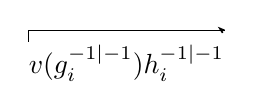
\begin{tikzpicture}[baseline=(prod.base)]
\node[inner sep=0pt] (prod) {$v(g_i^{\unsure{\deleted{\unsure{-1}}|\unsure{-1}}})h_i^{\unsure{\deleted{\unsure{-1}}|\unsure{-1}}}$};
\draw[line width=0.4pt] ([yshift=1pt]prod.north west) -- ([yshift=5pt]prod.north west) -- ([yshift=5pt]prod.north east);
\draw[line width=0.6pt] ([yshift=5pt]prod.north east) -- ++(-0.06,0.025) -- ++(0.035,-0.055);
\end{tikzpicture}}\bigr)l_i^{pq}
\]
Si on désigne par $S\overset{\unsure{\sim|\deleted{\sim}}}{\widehat{\widehat{\mathcal E}}}^!$ l'extension de $\widehat{\widehat{\mathcal E}}^!$ par $\hat{\mathbb Z}^{\{0,1,\infty\}}$ définie \deleted{\unsure{par le couple|par le groupe}} groupe des\unsure{.} \deleted{couples} triples d'un $u\in\widehat{\widehat{\mathcal E}}^!$ et d'un système de $g_i$ qui explicitent \inserted{via (21)} l'isomorphisme de la structure à lacets ($p$ étant le multiplicateur), on a sur $S\overset{\unsure{\sim|\deleted{\sim}}}{\widehat{\widehat{\mathcal E}}}^!$ trois fonctions à valeurs dans $\deleted{\unsure{\mathcal E}}\hat\Pi$
\[
(u,(g_i))\overset{\gamma_i}{\longmapsto}g_i,
\]
et on aura
\[
(24)\quad\gamma_i(\tilde v\tilde u)=\deleted{\unsure{\tilde v(\tilde u_i(\tilde u))\cdot\gamma_i(\tilde v)|\tilde v(\gamma_i(\tilde u))\cdot\gamma_i(\tilde v)}}\inserted{\deleted{\unsure{\gamma_i(\tilde v)\cdot v(\gamma_i(\tilde u))}} \tilde v(\gamma_i(\tilde u)\gamma_i(\tilde v)}
\]
i.e. $(\gamma_i)$ est un 1-cocycle sur le groupe \deleted{$\unsure{\widehat{\widehat{\mathcal E}}^!}$}\inserted{$S\overset{\unsure{\sim|\deleted{\sim}}}{\widehat{\widehat{\mathcal E}}}^!$} à valeurs dans le groupe \deleted{\unsure{produit du groupe}}\inserted{opposé au groupe} $\pi^{\{0,1,\infty\}}$.
\margin{\uline{NB} $S\widehat{\widehat{\mathcal E}}^!$ a été construit comme le groupe des Systèmes
\[
(p,g_0,g_1,g_\infty)\in\hat{\mathbb Z}^*\times\Pi^{\unsure{[0,1,\infty]|\{0,1,\infty\}}}
\]
satisfaisant la relation (22)}
\deleted{groupe}
Le sous-groupe de $S\widehat{\widehat{\mathcal E}}^!$ noyau de $S\overset{\unsure{\sim|\deleted{\sim}}}{\widehat{\widehat{\mathcal E}}}^!\longrightarrow\operatorname{Aut}\operatorname{ext}_{\mathrm{lac}}^!(\widehat{\unsure{\pi|\Pi}})$ s'identifie au groupe produit
\[
\left(\hat\Pi\times\prod_{i\in\{0,1,\infty\}}L_i\right)\simeq\widehat{\unsure{\pi|\Pi}}\times\underset{\begin{tikzpicture}[x=0.10cm,y=0.10cm,baseline=0ex]
\draw[line width=0.3pt] (0,1.35) -- (0.25,0) -- (0.65,1.25);
\draw[line width=0.3pt] (1.05,1.15) -- (1.15,0.1);
\fill (1.0,1.65) circle (0.08);
\end{tikzpicture}}{\unsure{(\hat{\mathbb Z})^{\{0,1,\infty\}}|(\hat{\mathbb Z})^3}}
\]
\mspage{24}
